%----------------------------------------------------------------------------------------
% ABSTRACT PAGE
%----------------------------------------------------------------------------------------
\startonleftwithgap
\newgeometry{top=0.5in, bottom=0.5in, left=0.5in, right=0.5in}
\pagestyle{plain}
\thispagestyle{empty}

\renewcommand{\familydefault}{\sfdefault} % Use sans-serif font throughout the document

\begin{tikzpicture}[remember picture, overlay]
    % Fill the triangle with the updated pattern
    \fill[pattern={Lines[angle=-45,distance={0.15cm}, line width=0.8pt]}, pattern color=greenTriangle]
        ([shift={(0,23.09cm)}]current page.south west) -- ++(0,4.19) -- ++(7.41,-2.095) -- cycle; % Triangle coordinates

\end{tikzpicture}

\begin{tabularx}{\textwidth}{X X} % Two equally spaced columns
  \centering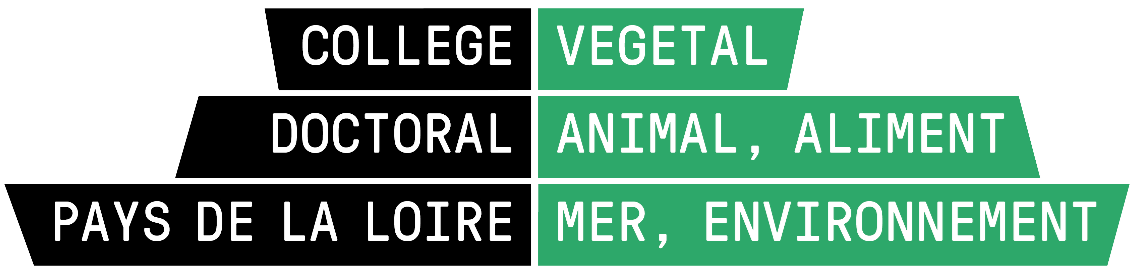
\includegraphics[height=2cm]{LogoED.png} & 
  \centering
\includegraphics[height=2cm]{LogoUN.jpg} \\
\end{tabularx} 

\vspace{1cm}

\noindent\textcolor[HTML]{2DA86A}{\rule{\textwidth}{5pt}}

\vspace{1cm}

\parbox{17cm}{

{{\fontsize{11}{15}\selectfont \textcolor{greenText}{\textbf{Titre :}}}}
{\fontsize{11}{15}\selectfont Caractérisation de la Végétation Intertidale sur les Côtes Européennes à l'Aide de la Télédétection Multi-Échelle en Réponse aux Pressions Naturelles et Anthropiques}} \\

{\fontsize{11}{15}\selectfont \textbf{Mots Clés:}}
{\fontsize{11}{15}\selectfont {Télédetection, Drones, Intertidale, Végétation, Multispectral}}

\parbox{17cm}{
\begin{multicols}{2}
{\fontsize{11}{15}\selectfont \textbf{Résumé:}}
{\fontsize{10}{14}\selectfont {La végétation intertidale joue un rôle clé dans les écosystèmes côtiers en stabilisant les sédiments, en abritant la biodiversité et en contribuant au cycle du carbone. Ce travail examine comment les approches de télédétection multi-échelles peuvent relever les défis de la surveillance et de la gestion de ces écosystèmes soumis à des pressions naturelles et anthropiques. En combinant des données issues de drones et de satellites, cette étude démontre l’efficacité de la télédétection multispectrale et hyperspectrale pour distinguer les zostères et les macroalgues dans les zones intertidales européennes. Les techniques d’apprentissage automatique sont mises en avant pour leur capacité à améliorer la précision des classifications et à relier les schémas de végétation aux gradients environnementaux, tels que l’altitude des marées et la stabilité des sédiments. Des expériences en laboratoire et des données de terrain soulignent l’impact des vagues de chaleur sur la santé de la végétation, fournissant des informations sur les réponses spectrales associées au stress et des indicateurs potentiels pour une détection précoce. Des analyses historiques révèlent également comment les activités humaines, telles que l’aquaculture, influencent la répartition de la végétation et la dynamique des écosystèmes au fil du temps. Cette approche intégrée souligne le potentiel de la télédétection pour capturer les schémas spatiaux et temporels de la biodiversité intertidale. Les résultats ont des implications majeures pour le suivi de la résilience des habitats, l’orientation des efforts de conservation et l’élaboration de politiques visant à atténuer les impacts du changement climatique et des activités humaines sur les environnements côtiers.}}
\end{multicols}
}

\noindent\textcolor[HTML]{2DA86A}{\rule{\textwidth}{5pt}}

\parbox{17cm}{

{{\fontsize{11}{15}\selectfont \textcolor{greenText}{\textbf{Title :}}}}
{\fontsize{11}{15}\selectfont Characterization of Intertidal Vegetation on European Coasts Using Multi-Scale Remote Sensing in Response to Natural and Anthropogenic Pressures}} \\

{\fontsize{11}{15}\selectfont \textbf{Keywords :}}
{\fontsize{11}{15}\selectfont {Remote Sensing, Drones, Intertidal, Vegetation, Multispectral}}

\parbox{17cm}{
\begin{multicols}{2}
{\fontsize{11}{15}\selectfont \textbf{Abstract :}}
{\fontsize{10}{14}\selectfont {Intertidal vegetation plays a key role in coastal ecosystems by stabilizing sediments, hosting biodiversity, and contributing to carbon cycling. This work examines how multi-scale remote sensing approaches can address challenges in monitoring and managing these ecosystems under natural and anthropogenic pressures. Combining drone and satellite data, this study demonstrates the effectiveness of multispectral and hyperspectral remote sensing in distinguishing seagrasses, macroalgae, across European intertidal zones. Machine learning techniques are highlighted for their ability to enhance classification accuracy and link vegetation patterns to environmental gradients, such as tidal elevation and sediment stability. Laboratory experiments and field data emphasize the impact of heatwaves on vegetation health, providing insights into the spectral responses associated with stress and potential metrics for early detection. Historical analyses further reveal how human activities, such as aquaculture, influence vegetation distribution and ecosystem dynamics over time. This integrated approach underscores the potential of remote sensing for capturing spatial and temporal patterns in intertidal biodiversity. The findings have broad implications for monitoring habitat resilience, guiding conservation efforts, and informing policies aimed at mitigating the impacts of climate change and human activities on coastal environments.}}
\end{multicols}
}

% \begin{tikzpicture}[remember picture, overlay]
%     % Fill the triangle with the updated pattern
%     \fill[pattern={Lines[angle=-45,distance={0.15cm}, line width=0.8pt]}, pattern color=greenTriangle]
%         ([shift={(21,1)}]current page.south west) -- ++(0,2.75) -- ++(-5.55,-1.375) -- cycle; % Triangle coordinates
% 
% \end{tikzpicture}
% 
% \begin{tikzpicture}[remember picture, overlay]
%     % Fill the triangle with the updated pattern
%     \fill[pattern=crosshatch dots, pattern color=greenTriangle]
%         ([shift={(0,1)}]current page.south east) -- ++(-5.55,0) -- ++(0,1.375) -- cycle; % Triangle coordinates
% \end{tikzpicture}

\restoregeometry